% The preceding line is only needed to identify funding in the first footnote. If that is unneeded, please comment it out.
\documentclass[conference]{IEEEtran}
\usepackage{fontspec}
\usepackage{amsmath,amssymb,amsfonts}
\usepackage{algorithmic}
\usepackage{graphicx}
\usepackage{textcomp}
\usepackage{xcolor}
\usepackage{comment}
\def\BibTeX{{\rm B\kern-.05em{\sc i\kern-.025em b}\kern-.08em
    T\kern-.1667em\lower.7ex\hbox{E}\kern-.125emX}}
\usepackage[numbers,sort&compress]{natbib}


\begin{document}

\title{How Does the Level of Somatosensory Feedback Fidelity Impact Motor Learning in VR: \\a Systematic Review}

\author{\IEEEauthorblockN{Reinprecht Christian}
\IEEEauthorblockA{TU Delft, NL \\
C.T.Reinprecht@student.tudelft.nl}
\and
\IEEEauthorblockN{Ratschat Alex}
\IEEEauthorblockA{TU Delft, NL \\
A.L.Ratschat@tudelft.nl}
\and
\IEEEauthorblockN{Marchal-Crespo Laura}
\IEEEauthorblockA{TU Delft, NL \\
L.MarchalCrespo@tudelft.nl}
}

\maketitle

\begin{abstract}
The abstract will come here. \\

\end{abstract}

\begin{IEEEkeywords}
motor learning, fidelity, virtual reality, systematic review
\end{IEEEkeywords}

%%%%% INTRODUCTION %%%%%
\section{Introduction}

Simulations in virtual reality (VR) provide a comprehensive platform for users to acquire new skills and competencies, with applications ranging from physical therapy and rehabilitation to sports and industrial training, education, marketing, telerobotics, and research, as well as gaming and entertainment \cite{Wu2023TrainingReality, Oagaz2022PerformanceReality}. Furthermore, the virtual environment (VE) allows for the studying of complex skills, as well as the evaluation of the user's performance without giving up on experimental control, which facilitates the understanding of motor learning on a level that is not possible in the physical world \cite{Harris2021ExploringSimulator, Levac2019LearningReview}. Therefore it is not surprising that there is a great interest in VR-based training simulations, especially to teach skills that would otherwise have to be acquired in dangerous or sensitive environments, such as construction work, military training, or surgical operations \cite{Adami2021EffectivenessTeleoperation, Lele2013VirtualUtility, Qi2021VirtualScenario}.

When interacting with real-world objects, we rely not only on visual feedback but also on information obtained through the mechanoreceptors in our skin and muscles \cite{Gonzalez-Grandon2021ProprioceptionInteraction}. To provide these stimuli in the virtual world, tools or devices are required to reproduce the sensations we would expect when interacting with objects in the VE, which includes the perception of pressure, vibration, temperature, and the position and movement of body parts. Exposing the user to these sensations when they are interacting with objects in VR --- generally denoted as somatosensory feedback --- may offer a promising approach to increase the effectiveness of motor learning \cite{Sainburg2022MovementNeurorehabilitation, Sigrist2013AugmentedReview}.
The degree to which the feedback in the VE mimics real-world interaction is determined by its fidelity \cite{Caird1996PersistentTraining}, which ranges from simple, binary cues such as vibration to high-fidelity feedback that feels as if the user is interacting with a real object \cite{Yang2023TheSimulation}.

% Teasing the research topic
While researchers previously assumed that higher fidelity correlates with better training performance in VR \cite{Caird1996PersistentTraining, Waller1998TheTraining}, as the interaction feels more natural, recent research suggests that there might be no linear correlation between the level of fidelity and motor performance: Instead, motor performance decreased in conditions that yielded mid-fidelity, compared to scenarios with high fidelity and well-designed low fidelity \cite{MahdiNabiyouni201520153DUI.}.

However, regarding task complexity, using a mid-fidelity controller may be beneficial, as it has been shown to effectively reduce the task load in a drilling task \cite{Yang2023TheSimulation}. This might be valuable for the motor learning performance of people with impaired motor skills \cite{Sigrist2013AugmentedReview}, aligning with the challenge point framework which states that less skilled subjects might not advance if the performed task is too demanding \cite{Guadagnoll2004ChallengeLearning}. \\

% Added reviews, second round of going to research gap
Extensive reviews have been conducted to illuminate the impact of haptic feedback in VR-based training \cite{Sigrist2013AugmentedReview} and the general utility of haptic simulation in motor learning \cite{Al-Saud2021TheReview}. However, it remains unclear how exactly different levels of haptic feedback fidelity affect motor learning, and to our knowledge, it has not been disentangled which kinds of tasks to be learned necessitate which degree of feedback accuracy.
Since supplying high fidelity to a VE is very costly, it is important to determine under which circumstances low-fidelity feedback, such as through somatosensory cues, is sufficient to increase the effectiveness of motor learning, and where high-fidelity feedback is necessary. 

In this work, we systematically review current research to create an overview of the impact of different levels of somatosensory feedback fidelity on motor learning in VR. Furthermore, this review will address how the level of feedback fidelity may affect the transfer of the learned skills to the real environment.

We hypothesize that in complex movements that necessitate precise timing for the correct execution of the task, such as ballistic movements, a high level of somatosensory feedback fidelity may be beneficial for motor learning. However, low-fidelity feedback may be sufficient for enhancing motor learning performance in scenarios involving constant movement velocities, allowing for reduced system cost and simpler experimental design. \newpage


%%%%% METHODS %%%%%
\section{Methods}

Several relevant articles were reviewed at the beginning to find eligible search terms. The query based on the research question consists of three main parts, namely \textit{virtual reality}, \textit{somatosensory feedback}, and \textit{motor learning}, each term with their respective synonyms. 

The final search query was as follows: motor AND (learning OR control OR training OR skills) AND (((virtual OR augmented) AND reality) OR ((remote OR virtual OR simulated) AND environment)) AND (((somatosensory OR haptic OR tactile OR proprioceptive OR kinesthetic OR cutaneous OR somatic) AND 
(cue* OR feedback OR rendering OR stimul*)) AND (fidelity OR realism OR accuracy OR precision OR exactness OR specificity)). The search terms were applied for the article title, abstract, and keywords.

Three databases (Scopus, IEEE Xplore, and PubMed) were searched in April 2024. Based on the required syntax of each database, the search query was slightly adapted. The exact search queries can be found in \ref{sec:queries}.
After removing the duplicates, the search yielded a total of 329 results.


\begin{figure}[ht]
    \centering
    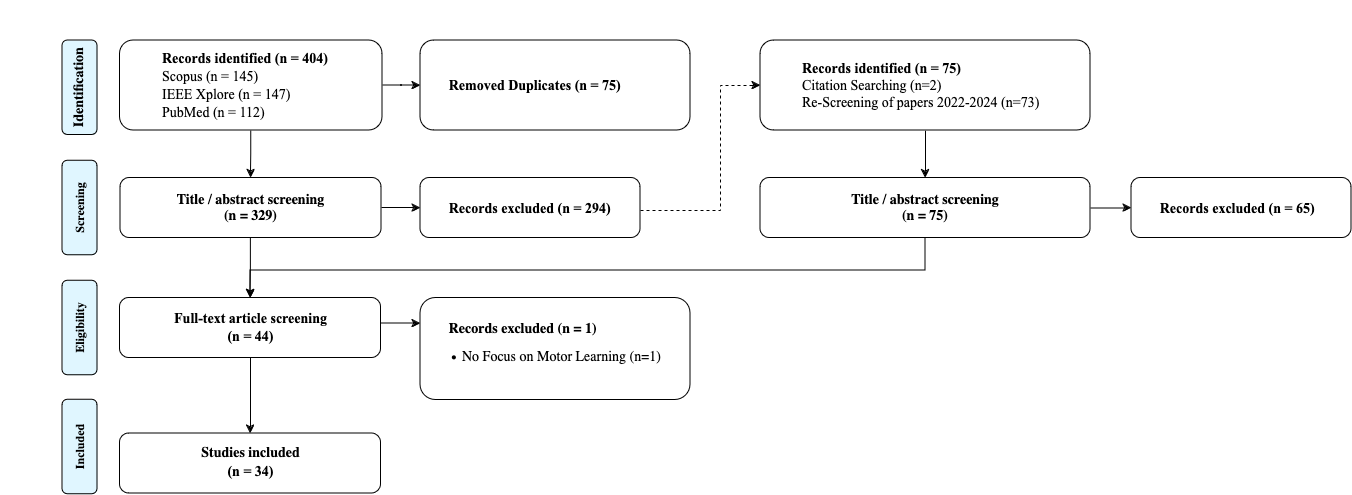
\includegraphics[width=\columnwidth]{prisma_overview.png} 
    \caption{Overview of the methodology using the PRISMA method}
    \label{fig:prisma}
\end{figure}

Following the PRISMA method \cite{Page2021TheReviews}, the found results were first screened based on their title and abstract and then reviewed in full length (see fig. \ref{fig:prisma}). After the first round, 

\subsection{Eligibility criteria}
\label{sec:eligibility}
\subsubsection{Inclusion criteria}
To be eligible for inclusion, studies needed to focus on the impact of haptic and/or somatosensory feedback on motor learning in humans. There were no publication date or language limits. 

\subsubsection{Exclusion criteria}
Studies were considered not eligible for inclusion if they were focused on:
\begin{itemize}
    \item Studies not related to motor learning in humans,
    \item Systems not providing haptic feedback in VR,
    \item Studies that focused on a neurological condition and its implications for motor learning,
    \item Studies explaining a new assessment system for the evaluation of motor learning.
\end{itemize}


\section*{Appendix}

\subsection{Queries}
\label{sec:queries}

\subsubsection{Scopus}
TITLE-ABS-KEY (motor AND (learning OR control OR training OR skills) AND (((virtual OR augmented) AND reality) OR ((remote OR virtual OR simulated) AND environment)) AND (((somatosensory OR haptic OR tactile OR proprioceptive OR kinesthetic OR cutaneous OR somatic) AND (cue* OR feedback OR rendering OR stimul*)) AND (fidelity OR realism OR accuracy OR precision OR exactness OR specificity)))

\subsubsection{IEEE Xplore}
motor AND (learning OR control OR training OR skills) AND (((virtual OR augmented) AND reality) OR ((remote OR virtual OR simulated) AND environment)) AND (((somatosensory OR haptic OR tactile OR proprioceptive OR kinesthetic OR cutaneous OR somatic) AND (cue* OR feedback OR rendering OR stimuli*)) AND (fidelity OR realism OR accuracy OR precision OR exactness OR specificity)) 

\subsubsection{PubMed}
motor AND (learning OR control OR training OR skills) AND (((virtual OR augmented) AND reality) OR ((remote OR virtual OR simulated) AND environment)) AND (((somatosensory OR haptic OR tactile OR proprioceptive OR kinesthetic OR cutaneous OR somatic) AND (cue OR cues OR feedback OR rendering OR stimuli*)) AND (fidelity OR realism OR accuracy OR precision OR exactness OR specificity))


\bibliographystyle{IEEEtran}
\bibliography{references}


\end{document}
